\documentclass[tikz,border=0pt]{standalone}
\usepackage[utf8]{inputenc}
\usepackage[T1]{fontenc}
\usepackage{lmodern}
\usepackage{amsmath,amssymb}
\usetikzlibrary{arrows.meta,positioning,fit,calc,backgrounds,shapes.geometric,decorations.pathreplacing}
\definecolor{navy}{HTML}{163A5F}
\definecolor{blue}{HTML}{2C6EAF}
\definecolor{lightblue}{HTML}{EAF2F8}
\definecolor{midblue}{HTML}{CFE1F2}
\definecolor{graytext}{HTML}{4A5560}
\definecolor{lightgray}{HTML}{F4F6F8}
\definecolor{green}{HTML}{3C8D73}
\definecolor{lightgreen}{HTML}{E8F5EF}
\definecolor{red}{HTML}{B24A4A}
\definecolor{lightred}{HTML}{FBEDEE}
\tikzset{
  title/.style={font=\sffamily\bfseries\fontsize{16}{18}\selectfont,text=navy,anchor=west},
  subtitle/.style={font=\sffamily\bfseries\fontsize{11}{13}\selectfont,text=navy},
  body/.style={font=\sffamily\fontsize{9.2}{11}\selectfont,text=graytext,align=left},
  small/.style={font=\sffamily\fontsize{8}{9.4}\selectfont,text=graytext,align=left},
  tinylabel/.style={font=\sffamily\fontsize{7.2}{8.4}\selectfont,text=graytext},
  panel/.style={rounded corners=3pt,draw=midblue,fill=white,line width=0.6pt},
  box/.style={rounded corners=2pt,draw=midblue,fill=lightblue,line width=0.6pt},
  worker/.style={rounded corners=2pt,draw=blue,dashed,line width=0.7pt,fill=white},
  task/.style={rounded corners=2pt,draw=blue,fill=lightblue,minimum width=0.85cm,minimum height=0.55cm,font=\sffamily\bfseries\small,text=navy},
  file/.style={draw=blue,fill=white,minimum width=0.55cm,minimum height=0.42cm,font=\sffamily\small,text=navy},
  arr/.style={-{Stealth[length=2.4mm,width=1.8mm]},draw=blue,line width=0.9pt},
  arrthin/.style={-{Stealth[length=2mm,width=1.5mm]},draw=blue,line width=0.7pt},
  arrred/.style={-{Stealth[length=2mm,width=1.5mm]},draw=red,dashed,line width=0.8pt},
  arrgreen/.style={-{Stealth[length=2mm,width=1.5mm]},draw=green,dotted,line width=1pt}
}
\begin{document}

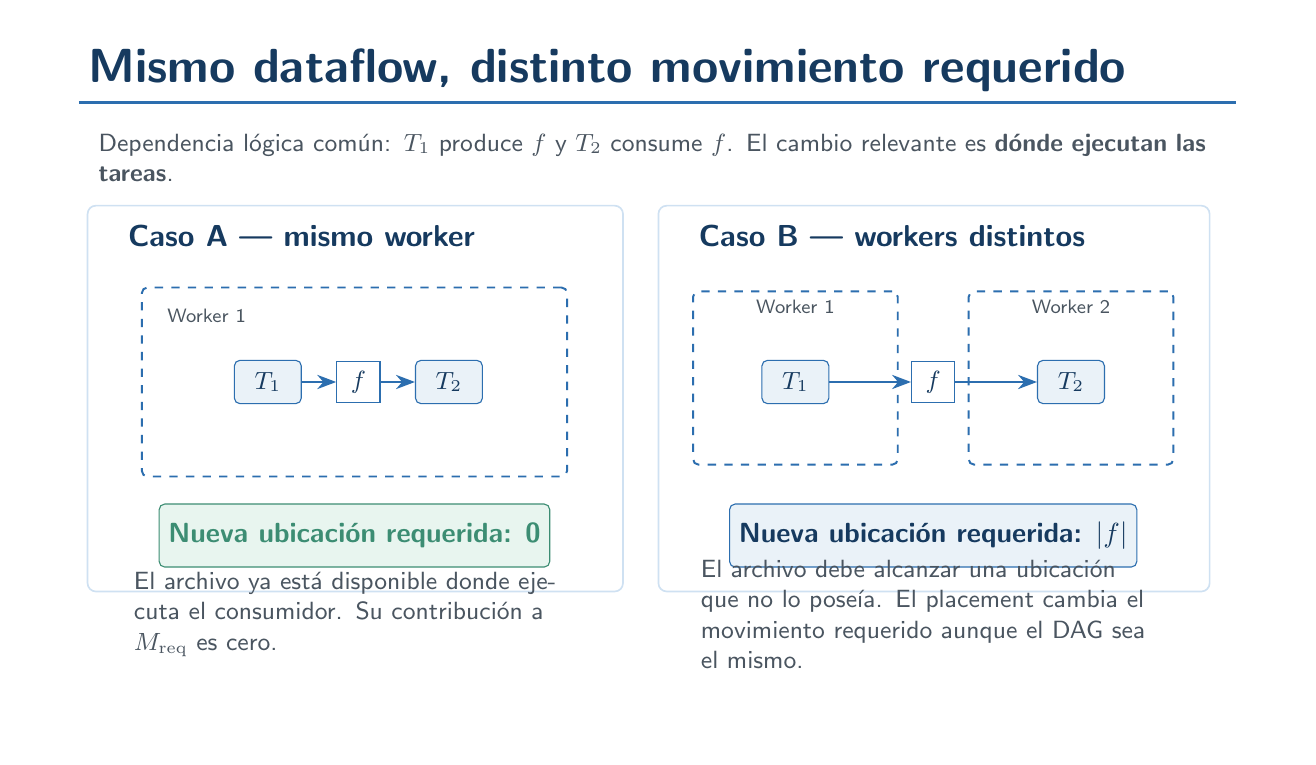
\begin{tikzpicture}[x=1cm,y=1cm]
\path[use as bounding box] (0,0) rectangle (16,9);
\node[title] at (0.65,8.45) {Mismo dataflow, distinto movimiento requerido};
\draw[blue,line width=1pt] (0.65,8.05)--(15.35,8.05);
\node[body,text width=14.2cm] at (8,7.35) {Dependencia lógica común: $T_1$ produce $f$ y $T_2$ consume $f$. El cambio relevante es \textbf{dónde ejecutan las tareas}.};
\node[panel,minimum width=6.8cm,minimum height=4.9cm,anchor=north west] at (0.75,6.75) {};
\node[subtitle,anchor=west] at (1.15,6.35) {Caso A — mismo worker};
\node[worker,minimum width=5.4cm,minimum height=2.4cm] at (4.15,4.5) {};
\node[tinylabel,anchor=north west] at (1.65,5.55) {Worker 1};
\node[task] (a1) at (3.05,4.5) {$T_1$}; \node[file] (af) at (4.2,4.5) {$f$}; \node[task] (a2) at (5.35,4.5) {$T_2$};
\draw[arr] (a1)--(af); \draw[arr] (af)--(a2);
\node[rounded corners=2pt,draw=green,fill=lightgreen,minimum width=4.3cm,minimum height=0.8cm,font=\sffamily\bfseries,text=green] at (4.15,2.55) {Nueva ubicación requerida: 0};
\node[body,text width=5.6cm] at (4.15,1.55) {El archivo ya está disponible donde ejecuta el consumidor. Su contribución a $M_{\mathrm{req}}$ es cero.};
\node[panel,minimum width=7.0cm,minimum height=4.9cm,anchor=north west] at (8.0,6.75) {};
\node[subtitle,anchor=west] at (8.4,6.35) {Caso B — workers distintos};
\node[worker,minimum width=2.6cm,minimum height=2.2cm] at (9.75,4.55) {}; \node[worker,minimum width=2.6cm,minimum height=2.2cm] at (13.25,4.55) {};
\node[tinylabel] at (9.75,5.45) {Worker 1}; \node[tinylabel] at (13.25,5.45) {Worker 2};
\node[task] (b1) at (9.75,4.5) {$T_1$}; \node[file] (bf) at (11.5,4.5) {$f$}; \node[task] (b2) at (13.25,4.5) {$T_2$};
\draw[arr] (b1)--(bf); \draw[arr] (bf)--(b2);
\node[rounded corners=2pt,draw=blue,fill=lightblue,minimum width=4.3cm,minimum height=0.8cm,font=\sffamily\bfseries,text=navy] at (11.5,2.55) {Nueva ubicación requerida: $|f|$};
\node[body,text width=5.9cm] at (11.5,1.55) {El archivo debe alcanzar una ubicación que no lo poseía. El placement cambia el movimiento requerido aunque el DAG sea el mismo.};
\end{tikzpicture}
\end{document}
